%%%%%%%%%%%%%%%%%%
% EE227A Project by Nathan Lam
%%%%%%%%%%%%%%%%%%


\documentclass{../../common/projectreport}

\usepackage{subfig}
\usepackage{graphicx}

\begin{document}

\section{Overview}

This section will review some applications using Robust PCA. Currently, most of the applications are related to computer vision. As we will show later, many images involve natural characteristic of low-rank structure, which makes Robust PCA a perfect fit to them. We will also explore some other applications that is theoretically with low-rank and sparse structure and show what we get from them. 

\section{Robust PCA Applications}

\subsection{Background modeling from surveillance video}

Video is a natural candidate for low-rank modeling, due to the correlation between frames. One of the most basic algorithmic tasks in video surveillance is to estimate a good model for the background variations in a scene. This task is complicated by the presence of foreground objects: in busy scenes, every frame may contain some anomaly. The background model needs to be flexible enough to accommodate changes in the scene, for example due to varying illumination In such situations, it is natural to model the background variations as approximately low rank. Foreground objects, such as cars or pedestrians, generally occupy only a fraction of the image pixels and hence can be treated as sparse errors.

\begin{figure}[hb]
  \centering
  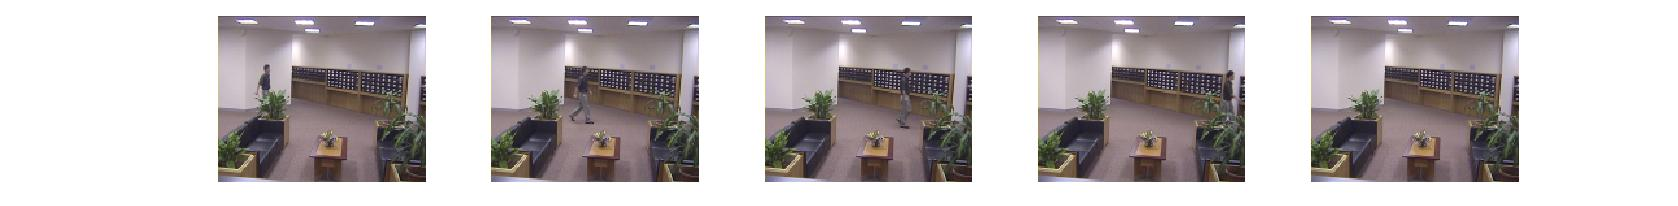
\includegraphics[width=1\textwidth]{SwitchLight_original.jpg}
  \caption{Original video frames}
  \label{fig:video:original}
\end{figure}

\begin{figure}[hb]
  \centering
  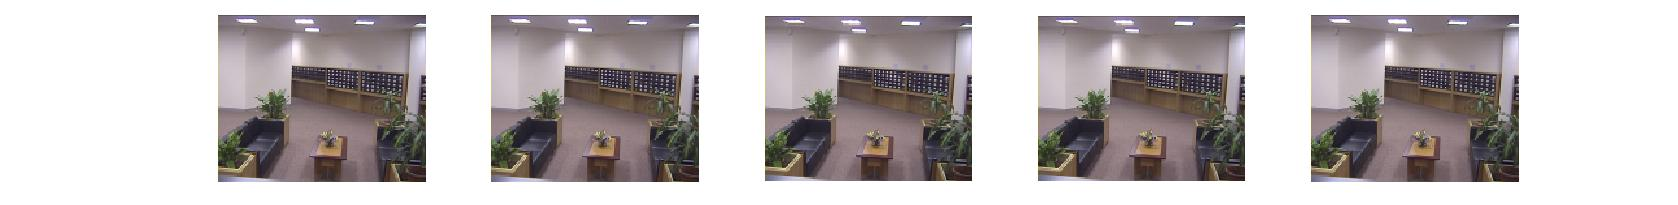
\includegraphics[width=1\textwidth]{SwitchLight_low_rank.jpg}
  \caption{Low-rank components}
  \label{fig:video:low_rank}
\end{figure}

\begin{figure}[hb]
  \centering
  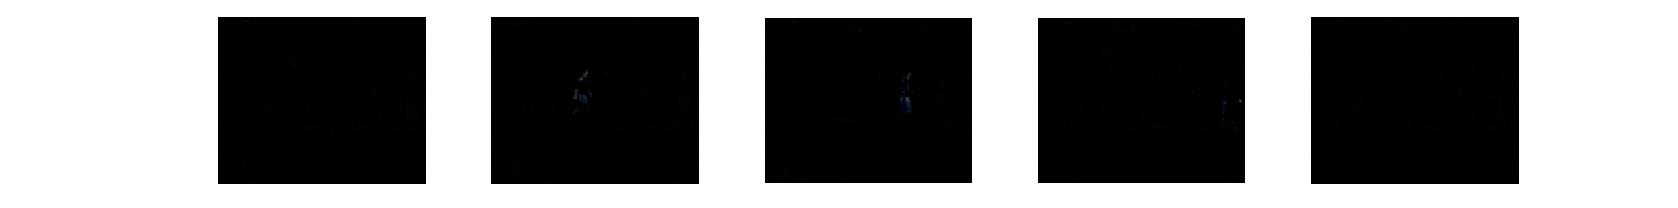
\includegraphics[width=1\textwidth]{SwitchLight_sparse.jpg}
  \caption{Sparse components}
  \label{fig:video:sparse}
\end{figure}

We consider five frames from an original video, as shown in fig.~\ref{fig:video:original}, which is a scenario that  one man passes by. The resolution of each frame is $176\times144$. We first separate them into three channels (RGB). For each channel, we stack each frame as a column  of our matrix $M\in\mathbb{R}^{25344\times5}$. We decompose $M$ into low-rank components $L$ and sparse components $S$ by Robust PCA. Then we combine the three channels again to form images with low-rank component and sparse components respectively. We are using a 2GHz qual core laptop and it takes 0.92s to finish decomposition for three channels. We can find that the $L$, as shown in fig.~\ref{fig:video:low_rank}, correctly recovers the background, while $S$, as shown in fig.~\ref{fig:video:sparse}, correctly identifies the moving person.

\subsection{Using Robust PCA in speech recognition}
Intuitively, a consistent sound would be of low-rank structure. If someone is speaking with background noise which is consistent, we would believe that we can separate a clearer speech (the sparse component) from background noise (low-rank component) via Robust PCA framework. If we get a clearer speech signal, the accuracy of speech recognition with current standard technique will increase. According to this thought, we did an experiment and try to see whether Robust PCA works in such case.

\begin{figure}[hb]
  \centering
  \subfloat[clean]{\label{fig:speech:clean}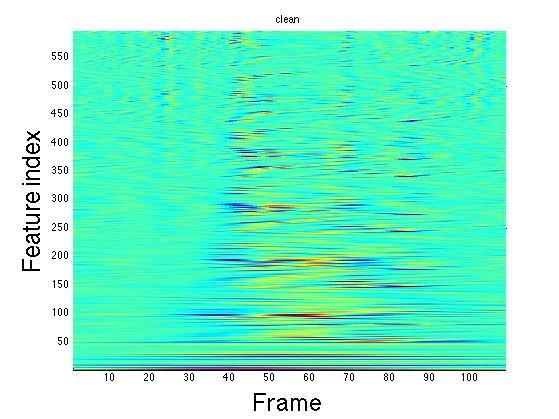
\includegraphics[width=0.5\textwidth]{speech_clean.jpg}}
  ~ %add desired spacing between images, e. g. ~, \quad, \qquad etc. (or a blank line to force the subfig onto a new line)
  \subfloat[noisy]{\label{fig:speech:noisy}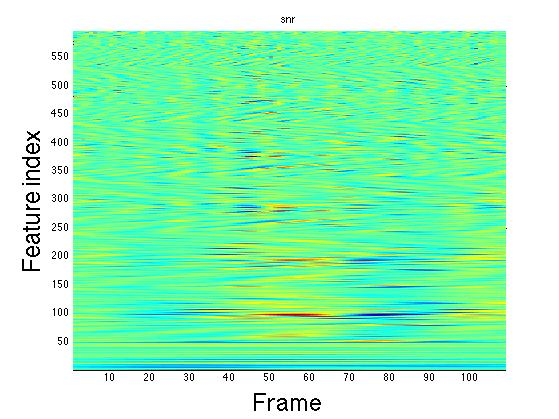
\includegraphics[width=0.5\textwidth]{speech_noisy.jpg}}
  ~ 
  \\ \subfloat[sparse]{\label{fig:speech:sparse}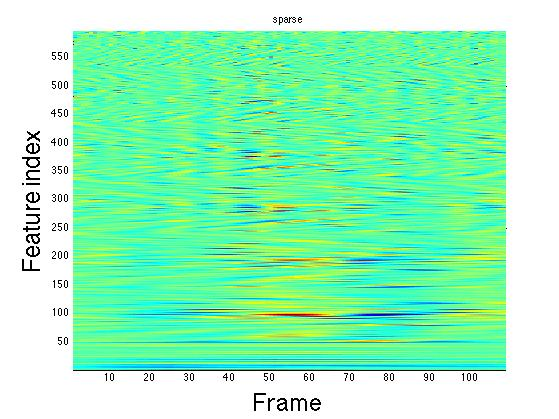
\includegraphics[width=0.5\textwidth]{speech_sparse.jpg}}
  ~
  \subfloat[low-rank]{\label{fig:speech:low_rank}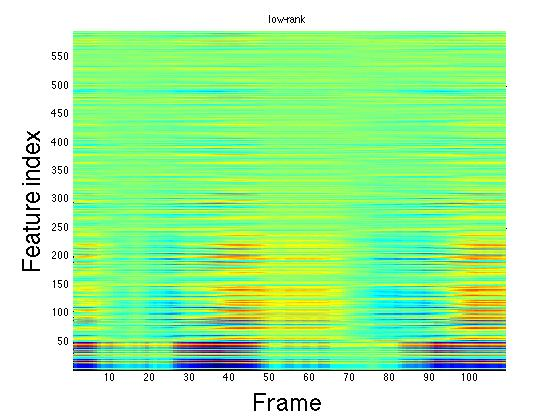
\includegraphics[width=0.5\textwidth]{speech_low_rank.jpg}}

  \caption{Speech features}
  \label{fig:speech}
\end{figure}

Figure~\ref{fig:speech:clean} shows the features of a clean speech signal, where the x-axis denotes indices of small time frames and the y-axis denote the features vectors at each frame. These features are computed by a standard method refering to \cite{}. Figure~\ref{fig:speech:noisy} shows the features domain of the same speech signal subjecting to noise with $SNR = 0$ in this case. We apply Robust PCA to decouple these features into low-rank component, as shown in fig.~\ref{fig:speech:low_rank}, and sparse component, as shown in fig.~\ref{fig:speech:sparse}. Technically, we would believe that sparse component is corresponding to our speech signal whereas low-rank component is corresponding to noise. Then we use the sparse component as new features and train a classifier via method in \cite{}. Unfortunately, comparing to the original method without  Robust PCA, we only got improvement in data set with subway noise, which we consider as the most consistent noise among the data set. In this data set, Robust PCA improve the accuracy rate with 3\% comparing to original method. For other noise, such as street noise and car noise, we both got decrease about 7\% in accuracy. One possible reason is that in the real world, most of the noise is not low-rank and they are not consistent. However, speech signal could be low-rank sometimes because there are only a limited vowels and consonants in a language, which makes Robust PCA not so suitable for de-noising.  

\section{Discussion}
Robust PCA framework is a powerful tool to separate low-rank components and sparse components if we are given a combination of these two structures. However, generally most of the real world data is not directly a combination of these two structures unless the data is subjected to some kinds of transformation. One example is the data set of human faces with different expressions and illuminations. In this case, some researches have proposed some methods, RASL~\cite{Peng:2010} and TILT~\cite{Zhang:2011}, based on the original convex optimization problem in Robust PCA. They introduce transformation parameters to the original framework and by linearizing with respect to the transformation parameters, we got a new but not difficult convex problem. As long as the data is within a certain degree of transformation, the algorithms can still recover the low-rank structure and sparse structure.

We can also observe that is image data, the sparse noise is always presented as blocks. For example, the person in fig.~\ref{fig:video:sparse} appears in connected pixels, so the noise is not distributed randomly in pixels. A possible direction that can improve the separation in image data is that we can introduce a penalty term in the original optimization problem:
\begin{align}
\begin{split}
p^* = \min_{L,S} \; &||L||_{*} + \lambda \||S||_{1} + \beta\sum_{i, j\in\mathcal{N}(i)}^{} (S_{i} - S_{j})^2\\
\text{s.t.} \quad &M = L+S
\end{split}
\label{applications:discussion}
\end{align}
where $\mathcal{N}(i)$ means all the entries next to $i$ in matrix $S$. This problem is still convex so we can solve it via existing algorithm for convex optimization problems.

%%%%%%%%%%%%%%%%%%%%%%%%%%%%%%%%%%%%%
\bibliographystyle{abbrv}
\bibliography{../../common/applications}


\end{document}